\documentclass[]{article}

\usepackage[parfill]{parskip}

\usepackage{hyperref}

\usepackage{amssymb}

\usepackage{listings}

\usepackage{fixltx2e}

\usepackage{graphicx}

\usepackage[T1]{fontenc}

\usepackage[T1]{fontenc}

\usepackage{color}
 
\definecolor{codegreen}{rgb}{0,0.6,0}
\definecolor{codegray}{rgb}{0.5,0.5,0.5}
\definecolor{codepurple}{rgb}{0.58,0,0.82}
\definecolor{backcolour}{rgb}{0.95,0.95,0.92}
 
\lstdefinestyle{mystyle}{
    backgroundcolor=\color{backcolour},   
    commentstyle=\color{codegreen},
    keywordstyle=\color{magenta},
    numberstyle=\tiny\color{codegray},
    stringstyle=\color{codepurple},
    basicstyle=\footnotesize,
    breakatwhitespace=false,         
    breaklines=true,                 
    captionpos=b,                    
    keepspaces=true,                 
    numbers=left,                    
    numbersep=5pt,                  
    showspaces=false,                
    showstringspaces=false,
    showtabs=false,                  
    tabsize=2
}
 
\lstset{style=mystyle}

%\sectionfont{\fontsize{10}{10}\selectfont}


\begin{document}


\author{
		Harman Kumar\\
		2013CS10224		
		}

\title{Project Report}
\maketitle

\section{Testing}

\begin{flushleft}
	The testing of the algorithms was done on the following three kinds of graphs:
	\begin{enumerate}
	\item Very sparse: These graphs had the number of edges very close to the number of verices. \\
	\[ E = V + \epsilon\] \[\epsilon\leq100\] 
	
	\item Sparse graphs: The number of edges were comparable to the number of vertices.\\
	
	\[ E = V * \alpha\] \[\alpha\leq10\] 	
	
	\item Dense graphs: The number of edges was quadratic in the number of vertices.\\
	
	\[ E = V^2/ \alpha\] \[E \leq V*(V-1)/2\] 	
	
	\end{enumerate}
	
\end{flushleft}

\section{Results And Plots:}



\subsection{Very Sparse Graphs:}

	For very sparse graphs, \[ E \approx V\]\\
	Following are the time curves:
	
\begin{center}
	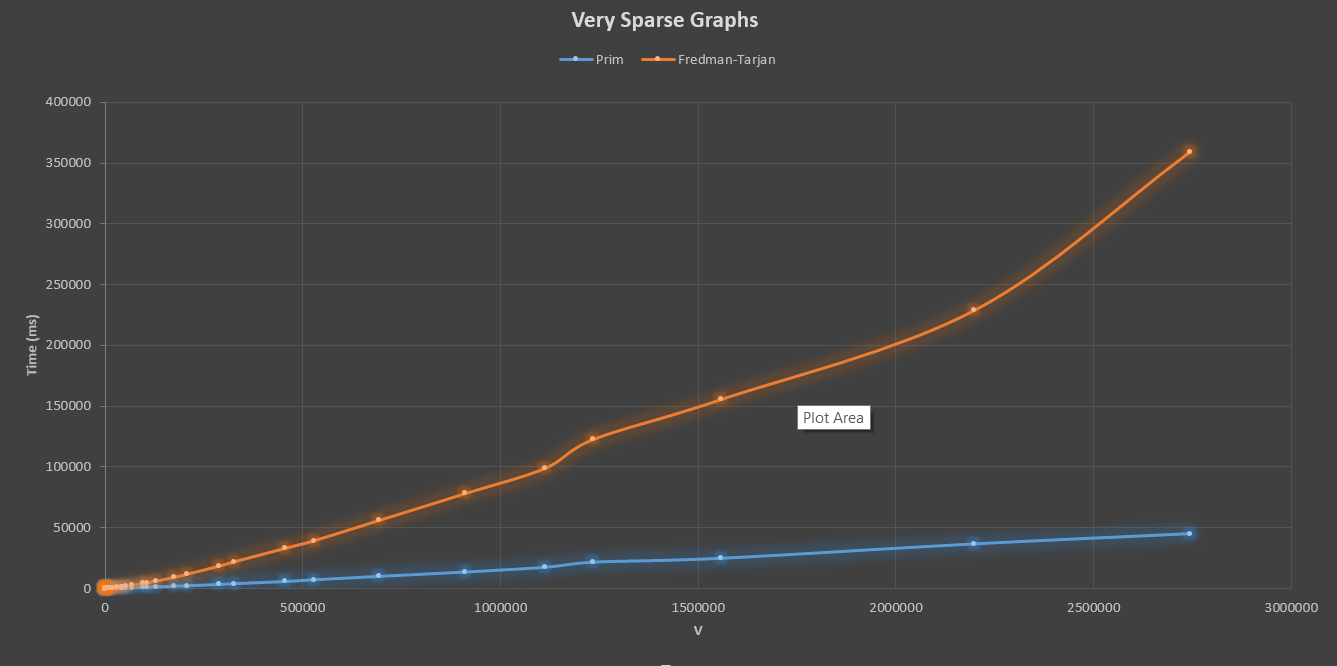
\includegraphics[width=12cm, height=8cm]{VerySparse_V.png}
	Time Vs. V
\end{center}


\begin{center}
	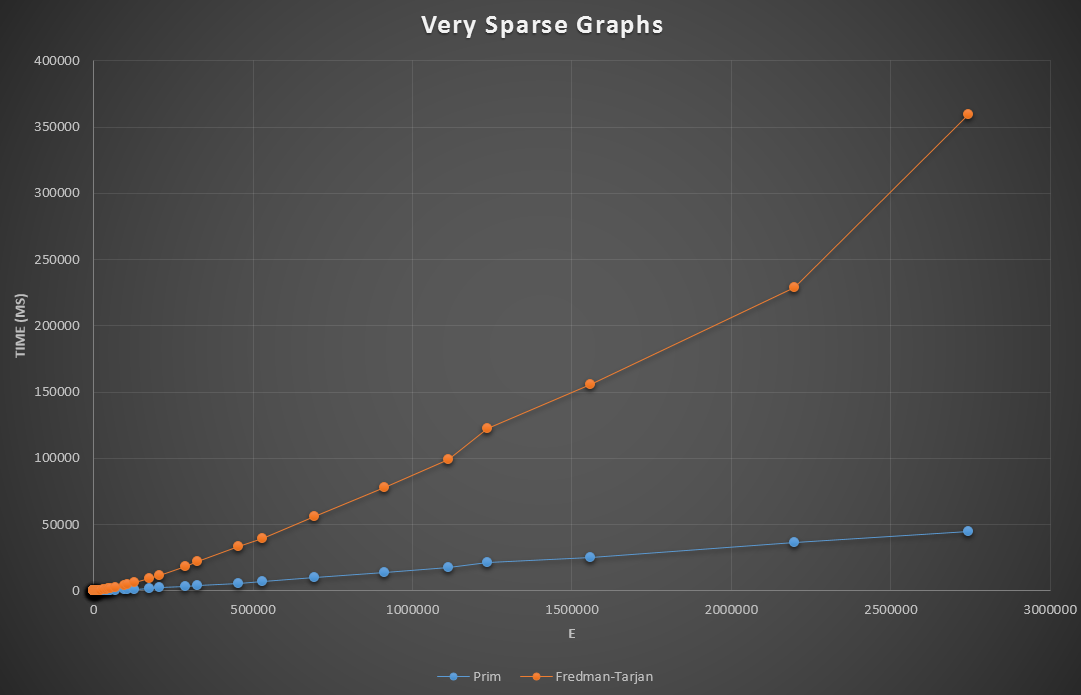
\includegraphics[width=12cm, height=8cm]{VerySparse_E.png}
	Time Vs. E
\end{center}

	Since $ E \approx V $, t is correlated with both V and E. 
			

\subsection{Sparse Graphs:}
For sparse graphs, \[ E = \theta(\alpha*V)\]
	
	Following are the time curves:


\begin{center}
	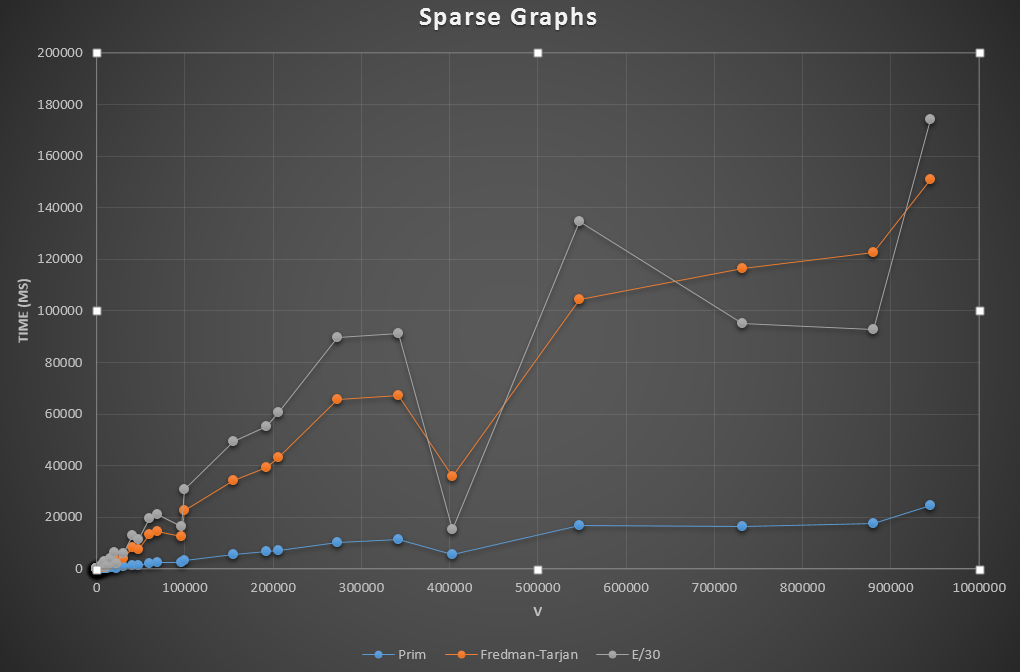
\includegraphics[width=12cm, height=8cm]{Sparse_V.png}
	Time Vs. V
\end{center}


\begin{center}
	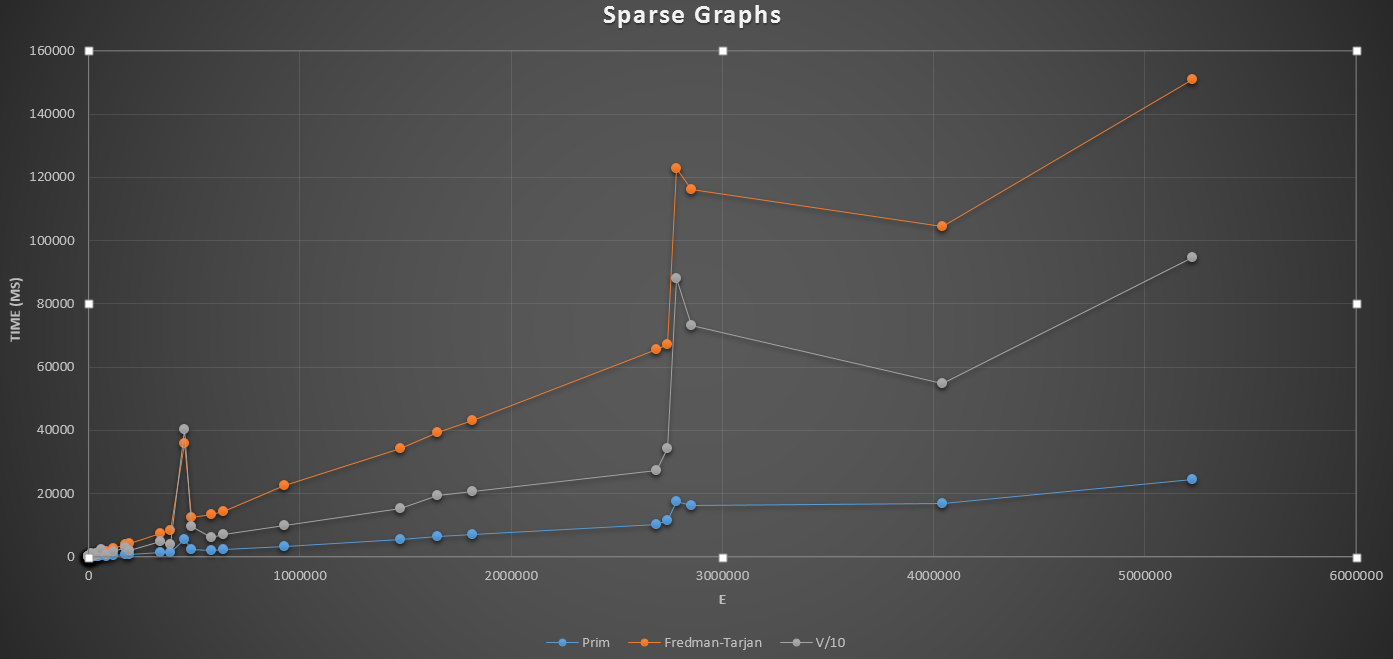
\includegraphics[width=12cm, height=8cm]{Sparse_E.png}
	Time Vs. E
\end{center}
	
	It could be seen that t is neither fully correlated with V, nor with E. 
			

\subsection{Dense Graphs:}

	For dense graphs, \[ E = \theta(V^2)\]
	
	Following are the time curves:


\begin{center}
	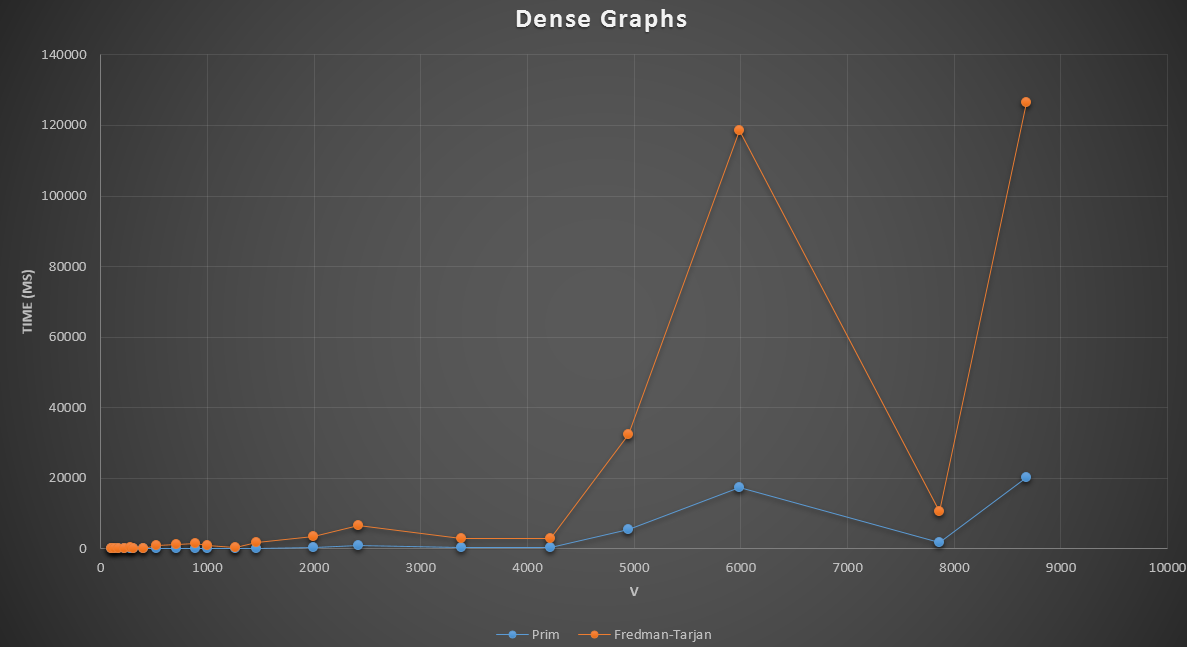
\includegraphics[width=12cm, height=8cm]{Dense_V.png}
	Time Vs. V
\end{center}


\begin{center}
	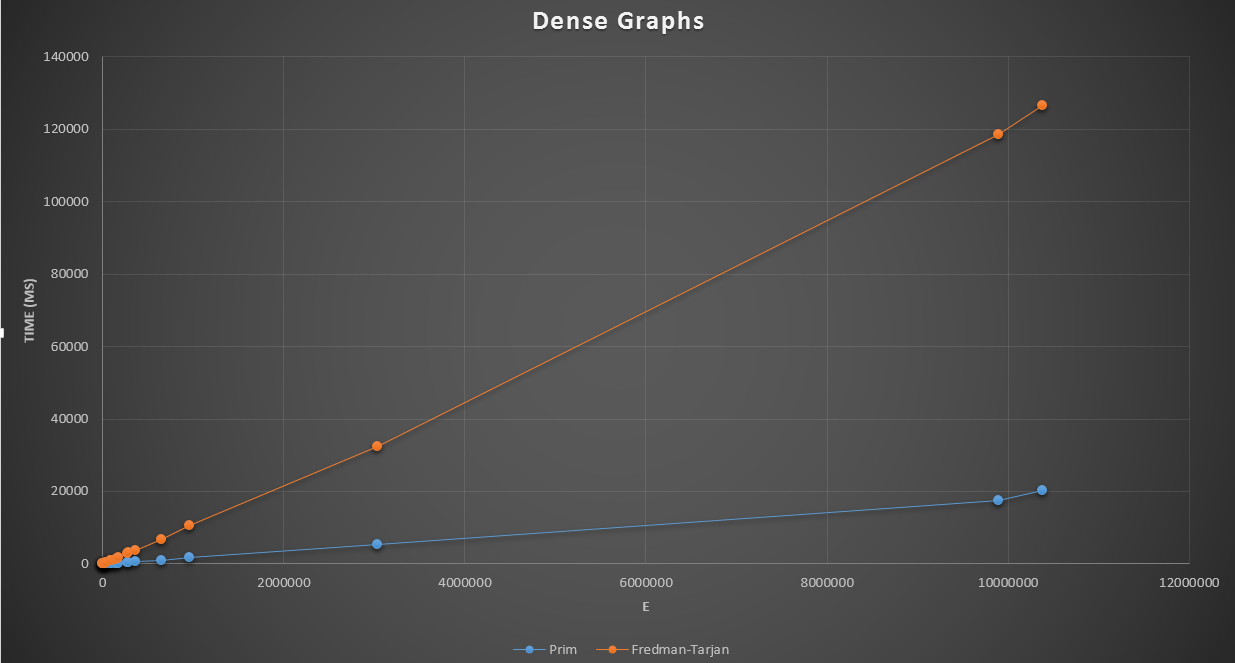
\includegraphics[width=12cm, height=8cm]{Dense_E.png}
	Time Vs. E
\end{center}


	
	It could be seen that there is no correlation between t and V, whereas t increases linearly with E.\\
			
	Time complexity for Prims Algorithm:
	\[ \theta(E + V\log(V)) \]
	
	Time complexity for Fredman-Tarjan Algorithm:
	\[ \theta(E\log^{*}(V))  \] 	
	
	Since, $E = \theta(V^2)$,
	E becomes the dominating factor in the time complexities and hence t starts to depend purely on E.

\section{Conclusion:}

\begin{enumerate}
	\item As the graph becomes dense, the correlation between V and time to compute MST decreases while the time complexity starts to depend more on E.

	\item It was seen that even for huge graphs, the Fredman-Tarjan algorithm using the fibonacci heap data structure took more time as compared to Prims algorithm, using the binary heap.
	
	\item The reason for the poor inferior performance of fredman-tarjan algorithm using the fibonacci heap is that Fibonacci heaps are slow and have significant storage overheads (4 pointers per node, plus a data field and a bool for housekeeping).
\end{enumerate}

\end{document}